\documentclass[tikz]{standalone}
% Diagonal positioning with one distance (M6, the owner's Venn finding):
% `above left=2.4cm of b` and `below right=of a` with a single node
% distance. Each case is tried on grid and off it, with the distance written
% after the key, coming from node distance, and from the default node
% distance; two distances ("and") are the control.
\usetikzlibrary{positioning}
\begin{tikzpicture}
  % Off grid: measured between borders.
  \node[draw, minimum size=10mm] (a) at (0,0) {};
  \node[draw, above left=24mm of a] (al) {al};
  \node[draw, below right=24mm of a] (br) {br};
  \node[draw, above right=12mm and 24mm of a] (ar) {ar};
  \node[draw, below left=of a] (bl) {bl};
  % On grid: between centers.
  \node[draw, minimum size=10mm] (g) at (8,0) {};
  \node[draw, on grid, above left=24mm of g] (gal) {gal};
  \node[draw, on grid, below right=24mm of g] (gbr) {gbr};
  \node[draw, on grid, above right=12mm and 24mm of g] (gar) {gar};
  \node[draw, on grid, below left=of g] (gbl) {gbl};
\end{tikzpicture}
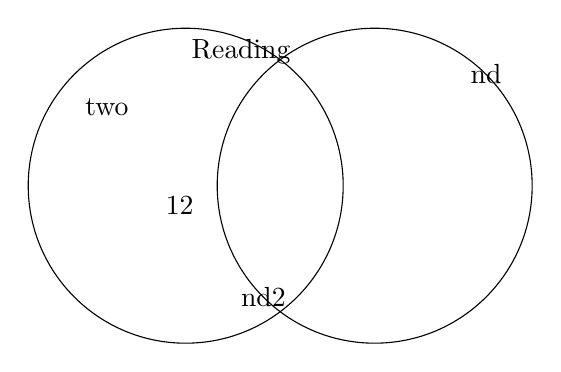
\begin{tikzpicture}[on grid, node distance=20mm]
  % The picture's on grid and a single node distance, as in the Venn template.
  \node[circle, draw, minimum size=40mm] (a) {};
  \node[circle, draw, minimum size=40mm, right=24mm of a] (b) {};
  \node[above left=2.4cm of b] (reading) {Reading};
  \node[below left=1.95cm and 7.8mm of reading] (onlya) {12};
  \node[above right=of b] (nd) {nd};
  \node[below left=of b, node distance=10mm and 30mm] (nd2) {nd2};
  \node[above left=1cm and 1cm of a] (two) {two};
\end{tikzpicture}
\begin{tikzpicture}[node distance=15mm]
  % Off grid, a single node distance in the picture's options.
  \node[draw] (a) {a};
  \node[draw, above right=of a] (b) {b};
  \node[draw, below left=of a] (c) {c};
  \node[draw, below left=5mm of a] (d) {d};
\end{tikzpicture}
\end{document}
